\chapter{Estudio del Problema}

Como se mencionó al final del capítulo anterior, la investigación vigente del fenómeno estudiado en el presente trabajo ha concluido en generar distintas hipótesis para explicar el mal rendimiento presentado por los sockets de internet en escenarios de concurrencia, más sin corroborar la validez de ninguna experimentalmente. Para ser exactos, y reiterando lo anterior, las sospechas se pueden agrupar en tres aristas distintas: Problemas de operación en primitivas del sistema, problemas de operación a nivel de canales de comunicación de hardware y problemas de operación en los mecanísmos de administración de recursos y balanceo de carga.

En el presente capítulo se estudian las tres líneas hipotéticas responsables del problema, inspeccionando en distintos niveles el funcionamiento del sistema, indagando en las operaciones teóricas de cada funcionamiento y contrastando dicho planteamiento a resultados experimentales obtenidos en cada caso. Es fruto de cada una de las siguientes subsecciones un análisis profundo del aspecto problemático estudiado, junto con una conclusión sobre el mismo. Así también, es fruto del presente capítulo un veredicto sobre cuales -Y en qué medida- de los problemas estudiados tienen verdadera responsabilidad en el fenómeno estudiado, de modo de confeccionar un marco de trabajo que nos permita empezar a postular enfoques de trabajo que paleen la problemática en cuestión.

\section{Estudio de Operación Primitivas de sincronización del Sistema}

La primera hipótesis a estudiar plantea que el bajo rendimiento de la operación de la interfaz de red -Ilustrada en nuestro caso de estudio por medio de sockets UDP- en escenarios de concurrencia, es causado por un mal desempeño de las estructuras que proveen los mecanismos de sincronización para dichos escenarios. Cómo se mencionó en el capítulo anterior, la capacidad multiprocesador de las computadoras modernas provee de un mayor poder de cómputo que se postula a ser aprovechado por medio del uso de técnicas de programación paralela, con el cuidado de que, en esos contextos de trabajo, los sistemas operativos deben estar preparados para atender situaciones de conflicto en el acceso a los recursos compartidos. Para éste propósito, se disponen de los mecanísmos de sincronización ya repasados en secciones anteriores que para estructuras de bajo nivel, cómo son los sockets de internet provistos por el propio sistema operativo- emplean el uso de mecanísmos de sincronización de bajo nivel como lo son los spinlocks, que protegen ciertas secciones de la estructura, tal y como se repasó en la sección XXXXX.

En éste caso, la priemra hipótesis describe que el causante del mal rendimiento al incorporar concurrencia en las lecturas a un socket es generado derechamente por dichas estructuras de protección en el acceso, situación causaría un fenómeno denominado \emph{Contención de Recurso}, que corresponde a un estado de conflicto en el acceso a un recurso compartido, producido por una situación de competencia en el acceso al mismo.

Para ratificar el planteamiento anterior, se hizo un estudio de llamadas a sistema siguiendo otros modelos de recopilación de datos ya evaluados \cite{slides:hpPerf} que permitiese vislumbrar la operación de las primitivas de sincronización operativas en el caso de estudio, a medida que se van agregando hilos de procesamiento, generando así un escenario de concurrencia, cómo se propuso desde un comienzo.

\subsection{Estudio de Llamadas de sistema}

La operación de las primitivas de sincronización que actúan en los procesos de bajo nivel del sistema operativo tienen la característica de estar determinadas por el uso de llamadas a funciones del sistema, ello pues es el mismo sistema operativo (o mejor dicho su núcleo) el que provee una interfaz simple para invocar dicha operación. Cómo son llamadas a sistema, es posible cuantificar cuando y cómo se realiazan las mismas, pudiendo modelar el proceso completo por medio de éste mecanismo.

Cómo en nuestro caso interesa estudiar el comportamiento de primitivas de sincronización de bajo nivel como son los spinlocks, se debe contemplar la API\footnote{Abreviatura de \emph{Application Programming Interface}, ó Interfaz de Programación de Aplicaciones en español.} con que trabaja el sistema para controlar éstas estructuras, ello pues, a pesar de que la estructura spinlock está bien definida, eisten distintas funciones que proveen variantes en el funcionamiento de los spinlocks, y dichos escenarios son presentables a lo largo de la ejecución del caso de prueba del estudio. El objetivo de éste estudio concierne un análisis cuantitativo de la cantidad de llamadas a sistema que sean bloqueantes sobre estructuras bloqueantes de tipo spinlock, y del tiempo que el sistema gasta en dichas condiciones.

En Linux los spinlocks se representan con estructuras \verb=spinlock_t= (incluidas en el archivo \verb= <linux/spinlock.h>=) que básicamente consisten en un campo de lock con un valor 1 (si está libre) o 0 (si está ocupado). Existen diversas funciones de atención que aplican distintos tipos de bloqueo \cite{book:spinlocks}:

\begin{description}
\item[void spin\_lock\_init(spinlock\_t *lock);] Inicializa una estructura spinlock y setea su valor inicial en 1.
\item[void spin\_lock(spinlock\_t *lock);] Es el bloqueo básico del sistema para tomar el lock. Consistente en la espera del lock hasta su valor 1 para luego setearlo en 0. Dicha espera se realiza con ciclos de \emph{busy-waiting} hasta que se brinde acceso. Es un bloqueo interrumpible por el sistema operativo, tanto por interrupciones de software como de hardware, dando paso a situaciones como que la CPU determine enviar el proceso responsable de la llamada a dormir por falta de recursos, memoria, etc.
\item[void spin\_lock\_irq(spinlock\_t *lock);] Bloqueo que deshabilita interrupciones del procesador local antes de adquirir el spinlock. Se debe cuidar de reactivar las interrupciones luego de liberado el lock.
\item[void spin\_lock\_irqsave(spinlock\_t *lock, unsigned long flags);] Similar a la operación de \verb=spin_lock_irq=, pero con la diferencia de que almacena el estado de interrupción previo en el valor \verb=flags=, de manera de que puede restablecerlo facilmente luego de liberar el lock.
\item[void spin\_lock\_bh(spinlock\_t *lock)] Similar a \verb=spin_lock_irq= con la diferencia de que sólo deshabilita las interrupciones de software, manteniendo habilitadas las interrupciones por hardware del sistema.
\item[int spin\_trylock(spinlock\_t *lock);] Para operaciones no bloqueantes para el uso de spinlocks. Retorna cero en caso de fallo al obtener el lock. No deshabilita interrupciones.
\item[bool mutex\_spin\_on\_owner(struct mutex *lock, struct task\_struct *owner)] Bloqueo que opera sobre una estructura de exclusión mutua (mutex) que utiliza el enfoque de \emph{Read-Copy-Update} (RCU), en donde los lectores son no bloqueantes. Ésta estructura tiene una sobrecarga menor que las anteriores; Sin embargo, las actualizaciones son más costosas ya que las versiones anteriores de la estructura de datos se deben guardar con el fin de dar cabida a los lectores ya existentes que se sincronizan a través de las barreras del mutex. Utilizando el enfoque de la RCU el bloqueo con esta estructura mutex asegura que la operación \emph{Test-and-Set} se ejecute en la misma CPU del propietario del lock, lo que reduce la cantidad de comunicación de memoria caché (y por consiguiente, el efecto de contención).
\end{description}

Asociadas a las anteriores llamadas de sistema están las variantes \verb=*_unlock*= que permiten liberar el elemento de bloqueo (seteando el valor del lock a 1) para recuperar así su disponibilidad para otros procesos.

Para poder rescatar las llamadas a sistema existen herramientas de software de bajo nivel, creados por los mismos desarrolladores del núcleo de Linux, que permiten realizar la tarea que nos proponemos en éste caso.

\subsubsection{Perf}
Perf \cite{slides:perfTools} o también llamado \emph{Perf\_events\footnote{Mayor documentación disponible en \url{https://perf.wiki.kernel.org/}}} es una herramienta de análisis de performance para entornos Linux. Corresponde a un subsistema del mismo kernel de Linux que provee todo un framework para el estudio de performance del sistema y de programas por medio de la captura de una amplia variedad de fuentes de datos. Perf es capaz de colectar datos por operatividad de software (contadores de software, \emph{tracepoints}, ejecución de funciones, paso a assembler, etc.) y también colectar información a nivel de hardware (manejo de PMU, lectura de \emph{Performance Counters}, etc.), características que lo postulan como uno de los sistemas más completos y flexibles para las tareas de profilling de aplicaciones y sistemas, y que lo hacen una buena herramienta para el actual estudio.

\begin{figure}[!h]
	\centering
	
\includegraphics[scale=.3]{imagenes/fcfm}
	\caption{Arquitectura de operación del framework provisto por \emph{Perf}.}
	\label{fig:perfFramework}
\end{figure}

Además de su gran capacidad para colectar datos, Perf es una herramienta de sencillo uso, pues su funcionamiento se basa en la supervisión de un determinado proceso o tarea de la cual construye un archivo con la información que se haya seleccionado a colectar \cite{article:perf}. Posteriormente, se pueden realizar operaciones de análisis más exhaustivo sobre dichos archivos de resultados.

El potencial de ésta herramienta la perfila como una utilidad indispensable para el estudio en cuestión. En primer lugar por su capacidad de análisis de ejecución de código que permite obtener información cuantificada de las llamadas a sistema y de la dinámica del árbol de llamados\footnote{Acá explicar brevemente que es un árbol de llamados} que permite reconocer la naturaleza de las funciones involucradas en el caso de estudio. En segunda instancia Perf es una estupenda herramienta para la recolección de datos de hardware al aprovechar el uso de la \emph{Performance Monitoring Unit} del hardware del sistema, una característica que será revisada en detalle en secciones posteriores.

\begin{figure}[!h]
	\centering
	
\includegraphics[scale=.3]{imagenes/fcfm}
	\caption{Esquema de captura de datos de un programa usando el comando \emph{perf-record}.}
	\label{fig:perfRecord}
\end{figure}

\subsubsection{FTrace}
Ftrace\footnote{Mayor documentación disponible en \url{http://elinux.org/Ftrace}} es otra poderosa herramienta para estudios de profiling disponible para sistemas Linux \cite{paper:FTraceSony}. Su funcionamiento opera de naturaleza muy intima con respceto al kernel mismo del sistema pues su recolección de datos se basa en el rastreo de la ejecución de funciones de forma dinámica en el espacio de kernel, lo que lo hace una estupénda utilidad para el estudio de llamadas al sistema, pudiendo recuperar datos como el tiempo de ejecución y cantidad de ocurrencia de las mismas.

Para su uso, FTrace opera como un verdadero framework del sistema sobre el kernel, del cual se pueden usar distintos métodos de rastreo de llamadas basados en distintos algoritmos. Una de las funciones más poderosas de FTrace es el resultado que se puede obtener por medio de la instrumentación de código, que se refiere a la práctica de incorporar a los programas a analizar \emph{tracepoints}, que son declaraciones explicitas de secciones de código a analizar y registrar. A pesar de que ésta característica es muy cómoda para programas propios, en el caso del análisis de funciones y llamadas de sistema la instrumentación de código es una característica obviable, siendo sólo necesaria la precisión de qué llamadas considerar en el análisis. El uso de ésta herramienta es muy flexible, siendo activable a disposición del usuario y conservando un registro de resultados. Además, FTrace es altamente configurable pudiendo explicitar filtros que usar como registros para las llamadas de sistema a analizar.

El provecho que se puede sacar de ésta herramienta es usar su capacidad para cuantificar tiempo de funciones del kernel para estudiar la atomicidad de las llamadas bloqueantes del sistema. Así por ejemplo, se pretende determinar el tiempo que se pasa en estados bloqueantes de spinlocks (de \emph{busy-waiting}) en los cuales sólo se pierde tiempo por caso de contención.


\subsection{Resultados}
Nos topamos con que las tendencias de tiempos son similares a las de los tiempos de esas llamadas, luego, hay una correlacion de esta estructura inhenrente al socket es la que causa el cuello de botella: indicio, el socket entero está siendo contenido por el spinlock de su estructura.

\subsubsection{Perf}
\subsubsection{FTrace}

\subsection{Análisis y Discusión de Resultados}
Aka un análisis general de los resultados en términis de gráficos obtenidos

\subsubsection{Call-Graph}
Una visualización de call-graph, quizá no como subseccion

\subsubsection{TraceDisplay}
Para poder obtener una interpretación adicional del fenómeno reconocido, se implementó una herramienta de visualziación de las llamadas a sistema para funciones de sincronización que permitiese reconocer las porciones de tiempo que tomaban en cada procesador dichas funciones. Para ello, la herramienta recibe un log de \emph{FTrace} con las llamadas de sistema yá filtradas y construye un mapa de tiempo coloreado, donde se pueden apreciar las porciones de tiempo que consumen las llamadas y desde que CPU se originan. El resultado se puede apreciar en la imagen \ref{fig:traceDisplay}. Éste subproducto de la investigación principal junto con su documentación de uso está publicado\footnote{Disponible en \url{https://github.com/sebablasko/TraceDisplay}} y disponible para su uso.

\begin{figure}[!h]
	\centering
	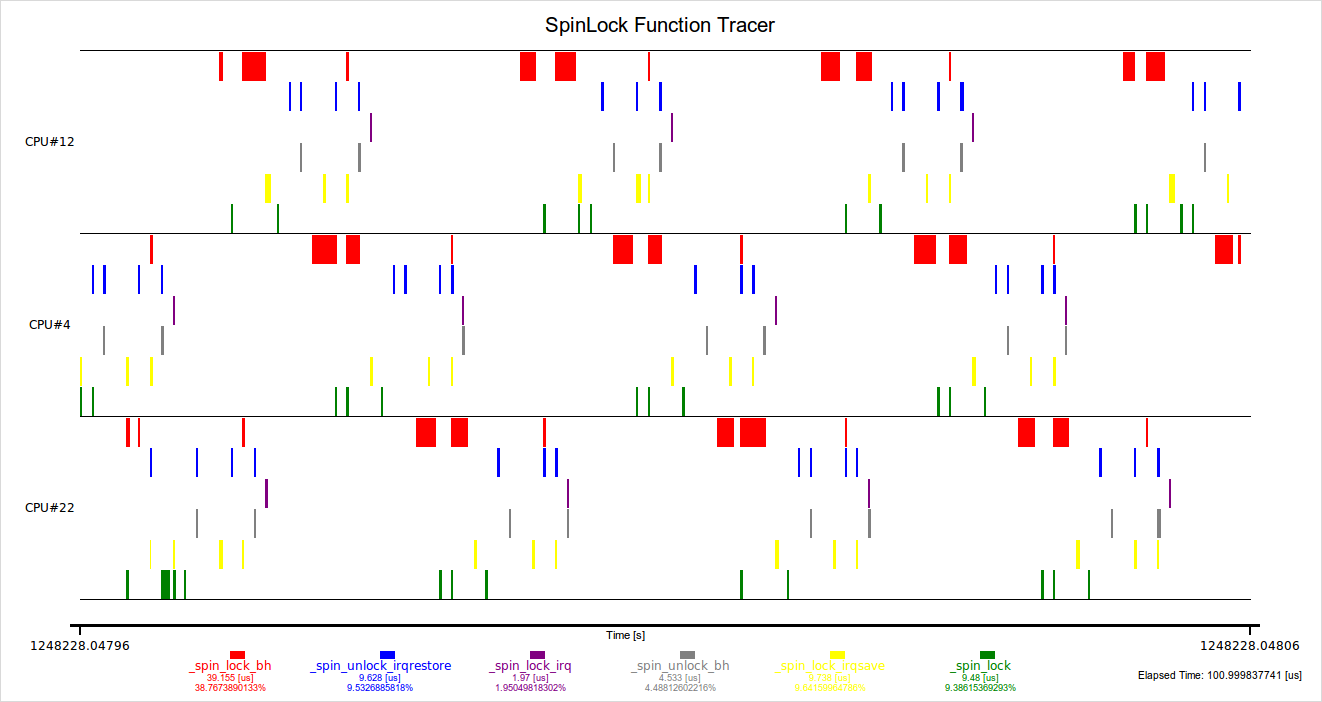
\includegraphics[scale=0.35]{imagenes/traceVisualization.png}
	\caption{visualización de aplicación de llamadas de sistema de sincronización realizadas entre procesadores, generada con la herramienta TraceDisplay desarrollada en el marco de éste trabajo. AKA FALTA EXPLICAR EL CASO EVALUADO}
	\label{fig:traceDisplay}
\end{figure}

AKA ME FALTA DECIR PARA QUE ME SIRVIO ESTA HERRAMIENTA



\section{Estudio de Canales de Comunicación de Hardware}
La segunda hipótesis para explicar la mala performance del caso de estudio presentado se centra en una componente de hardware más que de software. Cómo ya se mencionó, la capacidad multiprocesador de que se dispone en equipos modernos no es un recurso facil de aprovechar, de hecho, requiere una sofisticada operación y diseño tanto de las aplicaciones que solicitarán recursos, como del sistema operativo que ha de administrarlos. Como se repaso en secciones anteriores, en la práctica, la capacidad de paralelísmo viene dada gracias a un conjunto de protocolos y algoritmos de muy bajo nivel que coordinan y mantienen coherentes las componentes de datos para los diferentes procesadores \cite{paper:MESI, paper:snoop}, sin embargo, por muy sofisticados que dichos mecanismos sean, las nuevas tecnologías de hardware que prometen velocidades de trasnferencia y acceso nunca antes imaginiadas podrían significar un problema para éstas componentes.

Es precisamente en ésta línea que se establece la segunda hipótesis. En éste caso, se responsabiliza por el mal rendimiento a un problema de contención de recursos  nuevamente al spinlock de los sockets, pero ésta vez relacionado a la persistencia en el acceso al mismo y a la disponibilidad que se da del mismo a través de los mecanismos antes mencionados. En las arquitecturas modernas, los protocolos \emph{MESI} y de  \emph{SNOOP} son cruciales en la operación de ejecuciones paralelas para garantizar integridad en los datos, pero las arquitecturas mdoernas proponen nuevas distribuciones de los componentes internos de hardware, dotando de canales de mayor velocidad y reasignando los recursos. Ésta hipótesis plantea la posibilidad de que el degradamiento del caso de estudio sea causado por un fenómeno de \emph{Caché Bouncing}, que consiste en un 

En ésta línea, el fenómeno de \emph{Cache Bouncing} se podría acrecentar dada la arquitectura del sistema, la que al contemplar bancos de memoria distribuidos, algunos compartidos y otros exclusivos para los núcleos de procesamiento, podría estar manifestandose como resultado de las modificaciones concurrentes de los distintos procesadores sobre el socket, combinado a la operación de los protocolos de consistencia y correctitud para las lineas de caché del sistema.

\subsection{Características de Arquitecturas de Hardware Modernas}
\subsubsection{Arquitectura Intel QuickPath}

\subsection{Especificación y Captura de Eventos}
Performance counters are CPU hardware registers that count hardware events such as instructions executed, cache-misses suffered, or branches mispredicted. They form a basis for profiling applications to trace dynamic control flow and identify hotspots. perf provides rich generalized abstractions over hardware specific capabilities. Among others, it provides per task, per CPU and per-workload counters, sampling on top of these and source code event annotation.

\subsubsection{Resultados}
\subsubsection{Correlación de Eventos}
Para poder comprender mejor la tendencia de comportamiento en el experimento entre los distintos eventos capturados se repasaron posibles mecanismos de visualziación que permitieran una simple comparación entre dichas mediciones. Finalmente se optó por emplear una visualziación mediante el uso de una matriz de correlación, de manera de poder detectar facilmente conjuntos de eventos relacionados, ello combinando algúna estratégia de clusterización en el proceso de visualizar los datos. Ésta técnica es muy práctica y se ha empleado en otros escenarios sobre el mismo kernel en otras investigaciones con buenos resultados \cite{paper:clusteringKernel}.

\subsection{Análisis y Discusión de Resultados}

\section{Estudio de Distribución de Carga}
La tercera hipótesis de investigación plantea como responsable del mal rendimiento presentado en el caso de estudio al sistema de gestión y administración de tareas en el sistema operativo. En escenarios multicore como el estudiado, es normal que el sistema operativo realice como procedimiento de rutina la migración de procesos y la re-alocación de recursos y datos del sistema. Un caso práctico de ello es cuando un núcleo de procesamiento está sobreexigido y el sistema operativo redistribuye los hilos en dicho núcleo entre los procesadores disponibles del sistema, como una estratégia de balanceo de carga \cite{paper:NUMA}.

Ésta tercera hipótesis plantea que dicho proceso de reasignación de recursos sería perjudicial en escenarios de concurrencia basandose en que, mientras un proceso está en plena ejecución al incorporar más y más tareas en el mismo nucleo de procesamiento agregando hilos de ejecución, sería el sistema operativo quien comienzaría la reasignación automática de dichos hilos entre los distintos procesadores, cayendo en problemas como perdida de referencias de memoria en niveles de chacé primario de procesos en cuestión. En su peor escenario, ésta teoría lleva al conocido problema de \emph{caché bouncing} \cite{paper:cachebouncing} que corresponde al fenómeno de sobre corrección de los datos a nivel de lineas de cache de un procesador, producido por constantes cambios de contexto del \emph{scheduller} que genera migración de procesos. Un problema que ya se mencionó en el estudio de la sección previa.

Una alternativa que se ha estudiado para solventar éste problema es la técnica de \emph{Processor Affinity} que consiste en la asociación de tareas o procesos en procesadores especificos, de manera de controlar la ubicación de memoria y zona de ejecución del código. En otras palabras, se remueve la utilidad del mismo scheduler del sistema oeprativo para coordinar la mejor operación en la asignación de las mismas a las distintas CPU disponible, reemplazándolo por un criterio propio y estricto. Es una técnica muy interesante en el sentido de que, bien empleada puede proveer muy buenos resultados \cite{paper:cacheaffinity}, sin embargo también es facil degradar fuertemente el sistema al hacer mal uso de la misma.

\subsection{Processor Affinity}
\subsection{Esquemas de Distribución}
\subsection{Resultados Experimentales}
\subsection{Análisis y Discusión de Resultados}